%\documentclass{article}
\documentclass{article}
%\usepackage[utf8]{vietnam}
\usepackage[utf8]{inputenc}
\usepackage{anyfontsize,fontsize}
\changefontsize[13pt]{13pt}	
\usepackage{commath}
\usepackage{parskip,setspace}
\usepackage[table]{xcolor}
\usepackage{amssymb}
\usepackage[d]{esvect}
\usepackage[nottoc,notlot,notlof]{tocbibind}
\usepackage{slashed,cancel}
\usepackage{indentfirst,titlesec}
\usepackage{pdfpages}
\usepackage{graphicx,subcaption,floatrow,adjustbox,rotating}
\usepackage{nccmath}
\usepackage{mathtools}
\usepackage{amsfonts,esint}
\usepackage[printonlyused,withpage]{acronym}
\usepackage{wrapfig}
\usepackage[toc,page]{appendix}
\usepackage{amsmath,systeme}
\usepackage[thinc]{esdiff}
\usepackage{hyperref,tikz}
\usepackage{bm,physics,nicematrix}
% \usepackage[numbers,comma,sort&compress]{natbib}
%footnote
\usepackage{fancyhdr}
\usepackage{array,tocbibind}
\usepackage{enumitem}
\pagestyle{empty}


\usepackage{geometry}
\geometry{
	a4paper,
	total={170mm,257mm},
	left=20mm,
	top=20mm,
}



\newcommand{\image}[1]{
	\begin{center}
		\includegraphics[width=0.5\textwidth]{pic/#1}
	\end{center}
}




\renewcommand{\l}{\ell}
\newcommand{\dps}{\displaystyle}

\newcommand{\f}[2]{\dfrac{#1}{#2}}
\newcommand{\at}[2]{\bigg\rvert_{#1}^{#2} }


\renewcommand{\baselinestretch}{1.5}



\hypersetup{
	colorlinks=true,
	linkcolor=black,
	filecolor=magenta,      
	urlcolor=cyan,
	pdftitle={UT},
	citecolor=green,
	pdfpagemode=FullScreen,
}

\urlstyle{same}

\titleformat{\chapter}[display]
{\centering\large\bfseries} 
{\textbf{\MakeUppercase{\chaptername}} \ \thechapter\vspace{15pt}}{20pt}
{\large} 

%\newcommand{\thesistitlee}{Three-band tight binding model for TMD monolayers in the presence of a magnetic field}
\newcommand{\thesistitlee}{title}
\newcommand{\address}{NATIONAL UNIVERSITY OF HO CHI MINH CITY UNIVERSITY OF SCIENCE}
\newcommand{\department}{FACULTY OF PHYSICS - ENGINEERING PHYSICS}
\newcommand{\thesisauthor}{Tran Khoi Nguyen}
\newcommand{\thesisadvisor}{Your Advisor's Name}
\newcommand{\graddate}{Ho Chi Minh City, 2025}
\newcommand{\thesisdedication}{To all the Ph.D. pursuing brave souls}

\newlist{abbrv}{itemize}{1}
\setlist[abbrv,1]{label=,labelwidth=1in,align=parleft,itemsep=0.1\baselineskip,leftmargin=!}
\begin{document}
\setlength{\parindent}{20pt}
%\begin{titlepage}
%	\begin{center}
%		{\bfseries
%			
%			{\large {\bf \address}}\\
%			{{\textbf{\department}}}\\
%			{---------------------o0o--------------------}
%			\vspace{1.5cm}
%			
%			{\large {\bf UNDERGRADUATE THESIS}}\\
%			\vspace{3.0cm}
%			
%		}
%		
%	\end{center}
%	\textit{\textbf{\underline{Thesis title:}}}\\
%	\begin{center}
%		{\bfseries
%			
%			{\largerrr\thesistitlee}
%			\vspace{1in}
%			
%		}
%	\end{center}
%	\noindent
%	\makebox[\textwidth]{\hfill\makebox[3in]{\hrulefill}}\\
%	\begin{center}
%		\makebox[\textwidth]{\hfill\makebox[3in]{\hfill \textbf{Student: Tran Khoi Nguyen}\hfill}}
%		\makebox[\textwidth]{\hfill\makebox[3in]{\hfill \textbf{Supervisor: Dr. Huynh Thanh Duc}\hfill}}
%	\end{center}
%	\begin{tikzpicture}[remember picture, overlay]
%		\draw[line width=2pt]
%		([xshift=1.5cm, yshift=1.5cm] current page.south west)
%		rectangle
%		([xshift=-1.5cm, yshift=-1.5cm] current page.north east);
%	\end{tikzpicture}
%	\begin{center}
%		\vspace{2.5in}
%		{\graddate}
%	\end{center}
%\end{titlepage}
%\begin{titlepage}
%	\begin{center}
%		{\bfseries
%			
%			{\large {\bf \address}}\\
%			{{\textbf{\department}}}\\
%			\vspace{2.5cm}
%			
%			{\large {\bf UNDERGRADUATE THESIS}}\\
%			\vspace{3.0cm}
%			
%		}
%		
%	\end{center}
%	\textit{\textbf{\underline{Thesis title:}}}\\
%	\begin{center}
%		{\bfseries
%			
%			{\largerrr\thesistitlee}
%			\vspace{1in}
%			
%		}
%	\end{center}
%	\noindent
%	\makebox[\textwidth]{\hfill\makebox[3in]{\hrulefill}}\\
%	\begin{center}
%		\makebox[\textwidth]{\hfill\makebox[3in]{\hfill \textbf{Student: Tran Khoi Nguyen}\hfill}}
%		\makebox[\textwidth]{\hfill\makebox[3in]{\hfill \textbf{Supervisor: Dr. Huynh Thanh Duc}\hfill}}
%	\end{center}
%	\begin{center}
%		\vspace{2.5in}
%		{\graddate}
%	\end{center}
%\end{titlepage}
%
%\newpage
\pagenumbering{roman}
\pagestyle{fancy}
\renewcommand{\headrulewidth}{0pt}
\fancyhf{}
\fancyfoot[C]{\hspace{0cm} \thepage}
\setcounter{page}{1}
\pagenumbering{arabic}
\section{Theory}
\subsection{Three-band tight-binding model}
\noindent In the model introduced by Liu~\textit{et al.}, only the orbitals of the M atom are included. We denote the wave functions of the three orbitals of the M atom as
\begin{gather}
	\ket{\phi_{1}} = \ket{d_{z^{2}}} , \quad \ket{\phi_{2}} = \ket{d_{xy}} , \quad \ket{\phi_{3}} = \ket{d_{x^{2} - y^{2}}}.
\end{gather}
The Bloch wavefunction in this model has the form
\begin{gather}
	\psi_{\mathbf{k}}^{\lambda} (\mathbf{r}) = \sum_{j=1}^{3} C_{j}^{\lambda}(\mathbf{k}) \sum_{\mathbf{R}} e^{i \mathbf{k \cdot R}} \phi_{j}(\mathbf{r} - \mathbf{R}).
\end{gather}
The coefficents $C_{j}^{\lambda}(\mathbf{k})$ are the solutions of the eigenvalue equation
\begin{gather}
	\sum_{jj'}^{3} \left[H_{jj'}^{\text{TB}}(\mathbf{k}) - \varepsilon_{\lambda}(\mathbf{k}) S_{jj'}(\mathbf{k})\right] C_{j}^{\lambda}(\mathbf{k}) = 0,
\end{gather}
where
\begin{equation}
	\begin{aligned}
		H_{jj'}^{\text{TB}}(\mathbf{k}) = \sum_{\mathbf{R}} e^{i \mathbf{k \cdot R}} \bra{\phi_{j}(\mathbf{r})} H_{\text{1e}} \ket{\phi_{j'}(\mathbf{r - R})},
	\end{aligned}
\end{equation}
and
\begin{equation}
	\begin{aligned}
		S_{jj'}(\mathbf{k}) = \sum_{\mathbf{R}} \bra{\phi_{j}(\mathbf{r})} \ket{\phi_{j'}(\mathbf{r - R})} \approx \delta_{jj'}.
	\end{aligned}
\end{equation}

In the case $B \neq 0$, the wavefunction has an additional phase factor
\begin{gather}
	\psi_{\mathbf{k}}^{\lambda} (\mathbf{r}) = \sum_{j=1}^{3} C_{j}^{\lambda} \sum_{\mathbf{R}} e^{i \mathbf{k} \cdot \mathbf{R}} e^{i \theta_{\mathbf{R}} (\mathbf{r})} \phi_{j} (\mathbf{r} - \mathbf{R}),
\end{gather}
and choose $\theta = -\frac{e}{\hbar}\int_{\mathbf{r}}^{\mathbf{R}} \mathbf{A}(\mathbf{r}') \cdot d \mathbf{r}'$ as Peierls phase factor, the Hamiltonian now is
\begin{gather}
	H_{j  j' }^{} = \sum_{\mathbf{R}} e^{i \mathbf{k} \cdot \mathbf{R}} e^{\frac{ie}{\hbar} \int_{0}^{\mathbf{R}} \mathbf{A}(\mathbf{r}) \cdot d \mathbf{r}} E_{jj'} (\mathbf{R}),
\end{gather}
where
\begin{gather}
	E_{jj'} = \bra{\phi_{j}(\mathbf{r})} H_{1e} \ket{\phi_{j'} (\mathbf{r} - \mathbf{R})}.
\end{gather}
Using a uniform magnetic field $\mathbf{B} = (0,0,B)$ and Landau gauge $\mathbf{A} = (By,0,0)$. The Peierls hopping phase is given
\begin{equation}
	\begin{aligned}
		\frac{ie}{\hbar} \int_{\mathbf{0}}^{\mathbf{R}} \mathbf{A}(\mathbf{r}) \cdot d \mathbf{r} & = \frac{ie}{\hbar} \int_{\mathbf{0}}^{\mathbf{R}} B y dx \\
		                                                                                          & = \frac{ieB}{\hbar} \int_{0}^{1} y(\tau) x'(\tau) d\tau,
	\end{aligned}
\end{equation}
suppose that the atom M is located at lattice vector $\mathbf{R}_{m,n}$, the Peierls phase can be written as
\begin{gather}
	\theta_{m,n}^{m',n'} =
	\begin{cases}
		0                                                                             & \quad m' = m \pm 2, n' = n  ,      \\
		0                                                                             & \quad m' = m \pm 4, n' = n  ,      \\
		\pm \frac{e}{\hbar} \frac{B a^{2} \sqrt{3}}{2} m                              & \quad m' = m , n' = n \pm 2,       \\
		\pm \frac{e}{\hbar} \frac{B a^{2} \sqrt{3}}{4} \left(m \mp \frac{1}{2}\right) & \quad m' = m \mp 1, n' = n \pm 1 , \\
		\pm \frac{e}{\hbar} \frac{B a^{2} \sqrt{3}}{2} (m \mp 1)                      & \quad m' = m \mp 2, n' = n \pm 2,  \\
		\pm \frac{e}{\hbar} \frac{B a^{2} \sqrt{3}}{4} \left(m \mp \frac{3}{2}\right) & \quad m' = m \mp 3, n' = n \pm 1.  \\
	\end{cases}
\end{gather}
We obtain the Hamiltonian in magnetic field
\begin{equation}
	\begin{aligned}
		H_{jj'}^{\text{TB}}(\mathbf{k})
		 & = E_{jj'}(\mathbf{0}) + e^{i \mathbf{k} \cdot \mathbf{R}_{1}} E_{jj'}(\mathbf{R}_{1})
		+ e^{-i\pi(m + 1/2)\tfrac{\Phi}{\Phi_{0}}} e^{i \mathbf{k} \cdot \mathbf{R}_{2}} E_{jj'}(\mathbf{R}_{2})      \\
		 & + e^{-i\pi(m - 1/2)\tfrac{\Phi}{\Phi_{0}}} e^{i \mathbf{k} \cdot \mathbf{R}_{3}} E_{jj'}(\mathbf{R}_{3})
		+ e^{i \mathbf{k} \cdot \mathbf{R}_{4}} E_{jj'}(\mathbf{R}_{4})                                               \\
		 & + e^{i\pi(m - 1/2)\tfrac{\Phi}{\Phi_{0}}} e^{i \mathbf{k} \cdot \mathbf{R}_{5}} E_{jj'}(\mathbf{R}_{5})
		+ e^{i\pi(m + 1/2)\tfrac{\Phi}{\Phi_{0}}} e^{i \mathbf{k} \cdot \mathbf{R}_{6}} E_{jj'}(\mathbf{R}_{6})       \\
		 & + e^{- i\pi(m + 3/2)\tfrac{\Phi}{\Phi_{0}} } e^{i \mathbf{k} \cdot \mathbf{R}_{7}} E_{jj'}(\mathbf{R}_{7})
		+ e^{- 2i\pi m\tfrac{\Phi}{\Phi_{0}} } e^{i \mathbf{k} \cdot \mathbf{R}_{8}} E_{jj'}(\mathbf{R}_{8})          \\
		 & + e^{- i\pi(m - 3/2)\tfrac{\Phi}{\Phi_{0}} } e^{i \mathbf{k} \cdot \mathbf{R}_{9}} E_{jj'}(\mathbf{R}_{9})
		+ e^{ i\pi (m-3/2)\tfrac{\Phi}{\Phi_{0}} } e^{i \mathbf{k} \cdot \mathbf{R}_{10}} E_{jj'}(\mathbf{R}_{10})    \\
		 & + e^{2 i\pi m \tfrac{\Phi}{\Phi_{0}} } e^{i \mathbf{k} \cdot \mathbf{R}_{11}} E_{jj'}(\mathbf{R}_{11})
		+ e^{ i\pi (m+3/2)\tfrac{\Phi}{\Phi_{0}} } e^{i \mathbf{k} \cdot \mathbf{R}_{12}} E_{jj'}(\mathbf{R}_{12})    \\
		 & + e^{i \mathbf{k} \cdot \mathbf{R}_{13}} E_{jj'}(\mathbf{R}_{13})
		+ e^{-2i\pi(m + 1)\tfrac{\Phi}{\Phi_{0}}} e^{i \mathbf{k} \cdot \mathbf{R}_{14}} E_{jj'}(\mathbf{R}_{14})     \\
		 & + e^{-2i\pi(m - 1)\tfrac{\Phi}{\Phi_{0}}} e^{i \mathbf{k} \cdot \mathbf{R}_{15}} E_{jj'}(\mathbf{R}_{15})
		+ e^{i \mathbf{k} \cdot \mathbf{R}_{16}} E_{jj'}(\mathbf{R}_{16})                                             \\
		 & + e^{2i\pi(m - 1)\tfrac{\Phi}{\Phi_{0}}} e^{i \mathbf{k} \cdot \mathbf{R}_{17}} E_{jj'}(\mathbf{R}_{17})
		+ e^{2i\pi(m + 1)\tfrac{\Phi}{\Phi_{0}}} e^{i \mathbf{k} \cdot \mathbf{R}_{18}} E_{jj'}(\mathbf{R}_{18}),
	\end{aligned}
\end{equation}
where $\Phi_{0} = \frac{h}{e}$ and $\Phi = \frac{\sqrt{3}}{2} Ba^{2}$.
Since the Peierls phase depends on the the atomic position specified by the site indices $m,n$, the Hamiltonian is no longer invariant under translation of a primitive vector. For the case $\frac{\Phi}{\Phi_{0}} = \frac{p}{q}$, with $p,q \in \mathbb{Z}$, it is possible to restore the translational invariance if we expand the unit cell so that it includes $2q$ M atoms. We, then, define a new basis set of $6q$ atomic orbitals $\left\{ \phi_{j}(\mathbf{r} - \mathbf{R}_{m,n}) \right\}$. The wave function can be expressed as the coefficients of $C_{ji}^{\lambda}$ in the tight-binding wave function
\begin{gather}
	\psi_{\mathbf{k}}^{\lambda}(\mathbf{r}) = \sum_{j}^{3}\sum_{i}^{2q} C_{ji}^{\lambda}(\mathbf{k}) \sum_{{\mathbf{R}}} e^{\frac{ie}{\hbar}\int_0^{\mathbf{R} + \mathbf{R}_{i}}\mathbf{A}(\mathbf{r})\cdot d\mathbf{r}} e^{i\mathbf{k} \cdot (\mathbf{R} + \mathbf{R}_{i}) } \phi_{j}(\mathbf{r} - \mathbf{R} - \mathbf{R}_{i}).
\end{gather}
where $j = 1,2,3$ and $i$ labels the atom $\mathbf{R}_{i}$ in the magnetic unit cell, with $i = 1, \ldots, 2q$, and the new lattice vector now is $\mathbf{R} = k \mathbf{a}_{1} + l 2q \mathbf{a}_{2}$, where $k,l \in \mathbb{Z}$. In this basis, the TB Hamiltonian has an additional Peierls phase
\begin{gather}
	H_{j i  j' i'} = \sum_{\mathbf{R}} e^{i \mathbf{k} \cdot ( \mathbf{R} - \mathbf{R}_{i} + \mathbf{R}_{i'} )} e^{\frac{ie}{\hbar} \int_{\mathbf{R}_{i}}^{\mathbf{R} + \mathbf{R}_{i'}} \mathbf{A}(\mathbf{r}) \cdot d \mathbf{r}} \bra{\phi_{j}(\mathbf{r} - \mathbf{R}_{i})} H_{1e} \ket{\phi_{j'}(\mathbf{r} - \mathbf{R} - \mathbf{R}_{i'})},
\end{gather}
The sum over $\mathbf{R}$ include up to third-nearest-neighbor hoppings. It is remarkbly to note that the lattice vectors satisfying the condition $\abs{\mathbf{R}} \leq 2a$ are $\mathbf{R} = \mathbf{0}, \pm \mathbf{a}_{1}, \pm 2 \mathbf{a}_{1}$, we obtain the Hamiltonian
\begin{equation}
	\begin{aligned}
		 & H_{jnj'n'}^{\text{eff}}(\mathbf{k})
		= E_{jj'}(\mathbf{0}) \delta_{n,n'}
		+ e^{i\mathbf{k} \cdot \mathbf{R}_{1}}E_{jj'}(\mathbf{R}_{1}) \delta_{n,n'}
		+ e^{i\mathbf{k} \cdot \mathbf{R}_{4}}E_{jj'}(\mathbf{R}_{4}) \delta_{n,n'}                                                  \\
		 & + e^{-i\pi(m + 1/2)\frac{\Phi}{\Phi_{0}}}e^{i\mathbf{k} \cdot \mathbf{R}_{2}} E_{jj'}(\mathbf{R}_{2}) \delta_{n-1,n'}
		+ e^{-i\pi(m - 1/2)\frac{\Phi}{\Phi_{0}}} e^{i\mathbf{k} \cdot \mathbf{R}_{3}} E_{jj'}(\mathbf{R}_{3}) \delta_{n-1,n'}       \\
		 & + e^{i\pi(m - 1/2)\frac{\Phi}{\Phi_{0}}} e^{i\mathbf{k} \cdot \mathbf{R}_{5}} E_{jj'}(\mathbf{R}_{5}) \delta_{n+1,n'}
		+ e^{i\pi(m + 1/2)\frac{\Phi}{\Phi_{0}}} e^{i\mathbf{k} \cdot \mathbf{R}_{6}} E_{jj'}(\mathbf{R}_{6}) \delta_{n+1,n'}        \\
		 & + e^{- i\pi(m + 3/2)\frac{\Phi}{\Phi_{0}} } e^{i \mathbf{k} \cdot \mathbf{R}_{7}} E_{jj'}(\mathbf{R}_{7}) \delta_{n-1,n'}
		+ e^{- 2i\pi m\frac{\Phi}{\Phi_{0}} } e^{i \mathbf{k} \cdot \mathbf{R}_{8}} E_{jj'}(\mathbf{R}_{8}) \delta_{n-2,n'}          \\
		 & + e^{- i\pi(m - 3/2)\frac{\Phi}{\Phi_{0}} } e^{i \mathbf{k} \cdot \mathbf{R}_{9}} E_{jj'}(\mathbf{R}_{9}) \delta_{n-1,n'}
		+ e^{ i\pi (m-3/2)\frac{\Phi}{\Phi_{0}} } e^{i \mathbf{k} \cdot \mathbf{R}_{10}} E_{jj'}(\mathbf{R}_{10}) \delta_{n+1,n'}    \\
		 & + e^{2 i\pi m \frac{\Phi}{\Phi_{0}} } e^{i \mathbf{k} \cdot \mathbf{R}_{11}} E_{jj'}(\mathbf{R}_{11}) \delta_{n+2,n'}
		+ e^{ i\pi (m+3/2)\frac{\Phi}{\Phi_{0}} } e^{i \mathbf{k} \cdot \mathbf{R}_{12}} E_{jj'}(\mathbf{R}_{12}) \delta_{n+1,n'}    \\
		 & + e^{i \mathbf{k} \cdot \mathbf{R}_{13}} E_{jj'}(\mathbf{R}_{13}) \delta_{n,n'}
		+ e^{-2i\pi(m + 1) \frac{\Phi}{\Phi_{0}} } e^{i \mathbf{k} \cdot \mathbf{R}_{14}} E_{jj'}(\mathbf{R}_{14}) \delta_{n-2,n'}   \\
		 & + e^{-2i\pi(m - 1) \frac{\Phi}{\Phi_{0}}} e^{i \mathbf{k} \cdot \mathbf{R}_{15}} E_{jj'}(\mathbf{R}_{15}) \delta_{n-2,n'}
		+ e^{i \mathbf{k} \cdot \mathbf{R}_{16}} E_{jj'}(\mathbf{R}_{16}) \delta_{n,n'}                                              \\
		 & + e^{2i\pi(m - 1)\frac{\Phi}{\Phi_{0}}} e^{i \mathbf{k} \cdot \mathbf{R}_{17}} E_{jj'}(\mathbf{R}_{17}) \delta_{n+2,n'}
		+ e^{2i\pi(m + 1)\frac{\Phi}{\Phi_{0}}} e^{i \mathbf{k} \cdot \mathbf{R}_{18}} E_{jj'}(\mathbf{R}_{18}) \delta_{n+2,n'}.
	\end{aligned}
\end{equation}
where $\Phi_{0} = \frac{h}{e}$, $\Phi = \frac{\sqrt{3}}{2} Ba^{2}$ and $E(\mathbf{R})$ are obtained from Liu \textit{et al.}

\subsection{The cyclotron theory}
The cyclotron frequency can be obtained from the energy difference between two Landau levels
\begin{equation}
	\begin{aligned}
		\hbar \omega_{c} & = E_{n+1} - E_{n}  ,
	\end{aligned}
\end{equation}
which gives
\begin{equation}
	\begin{aligned}
		\omega_{c}  = \frac{E_{n+1} - E_{n}}{\hbar}.
	\end{aligned}
\end{equation}
On the other hand, the cyclotron frequency is also defined as
\begin{gather}
	\omega_{c}         = \frac{eB}{m^{*}}.
\end{gather}
Combining the two expressions, the effective mas can be written as
\begin{gather}
	m^{*}  =  \frac{eB}{\omega_{c}} = \frac{eB}{\frac{E_{n+1} - E_{n}}{\hbar}} = \frac{eB \hbar}{E_{n+1} - E_{n}},
\end{gather}
and
\begin{gather}
	\omega_{c} = \frac{E_{n+1} - E_{n}}{\hbar}.
\end{gather}
The radius of cyclotron orbit can be written as
\begin{gather}
	r_{c} = \frac{v_{F}}{\omega_{c}} = \frac{v_{F} \hbar}{E_{n+1} - E_{n}} = \frac{v_{F} m^{*}}{eB},
\end{gather}
where $v_{F}$ is given in Table 1.

\begin{figure}[htb]
	\begin{subfigure}{0.495\textwidth}
		\centering
		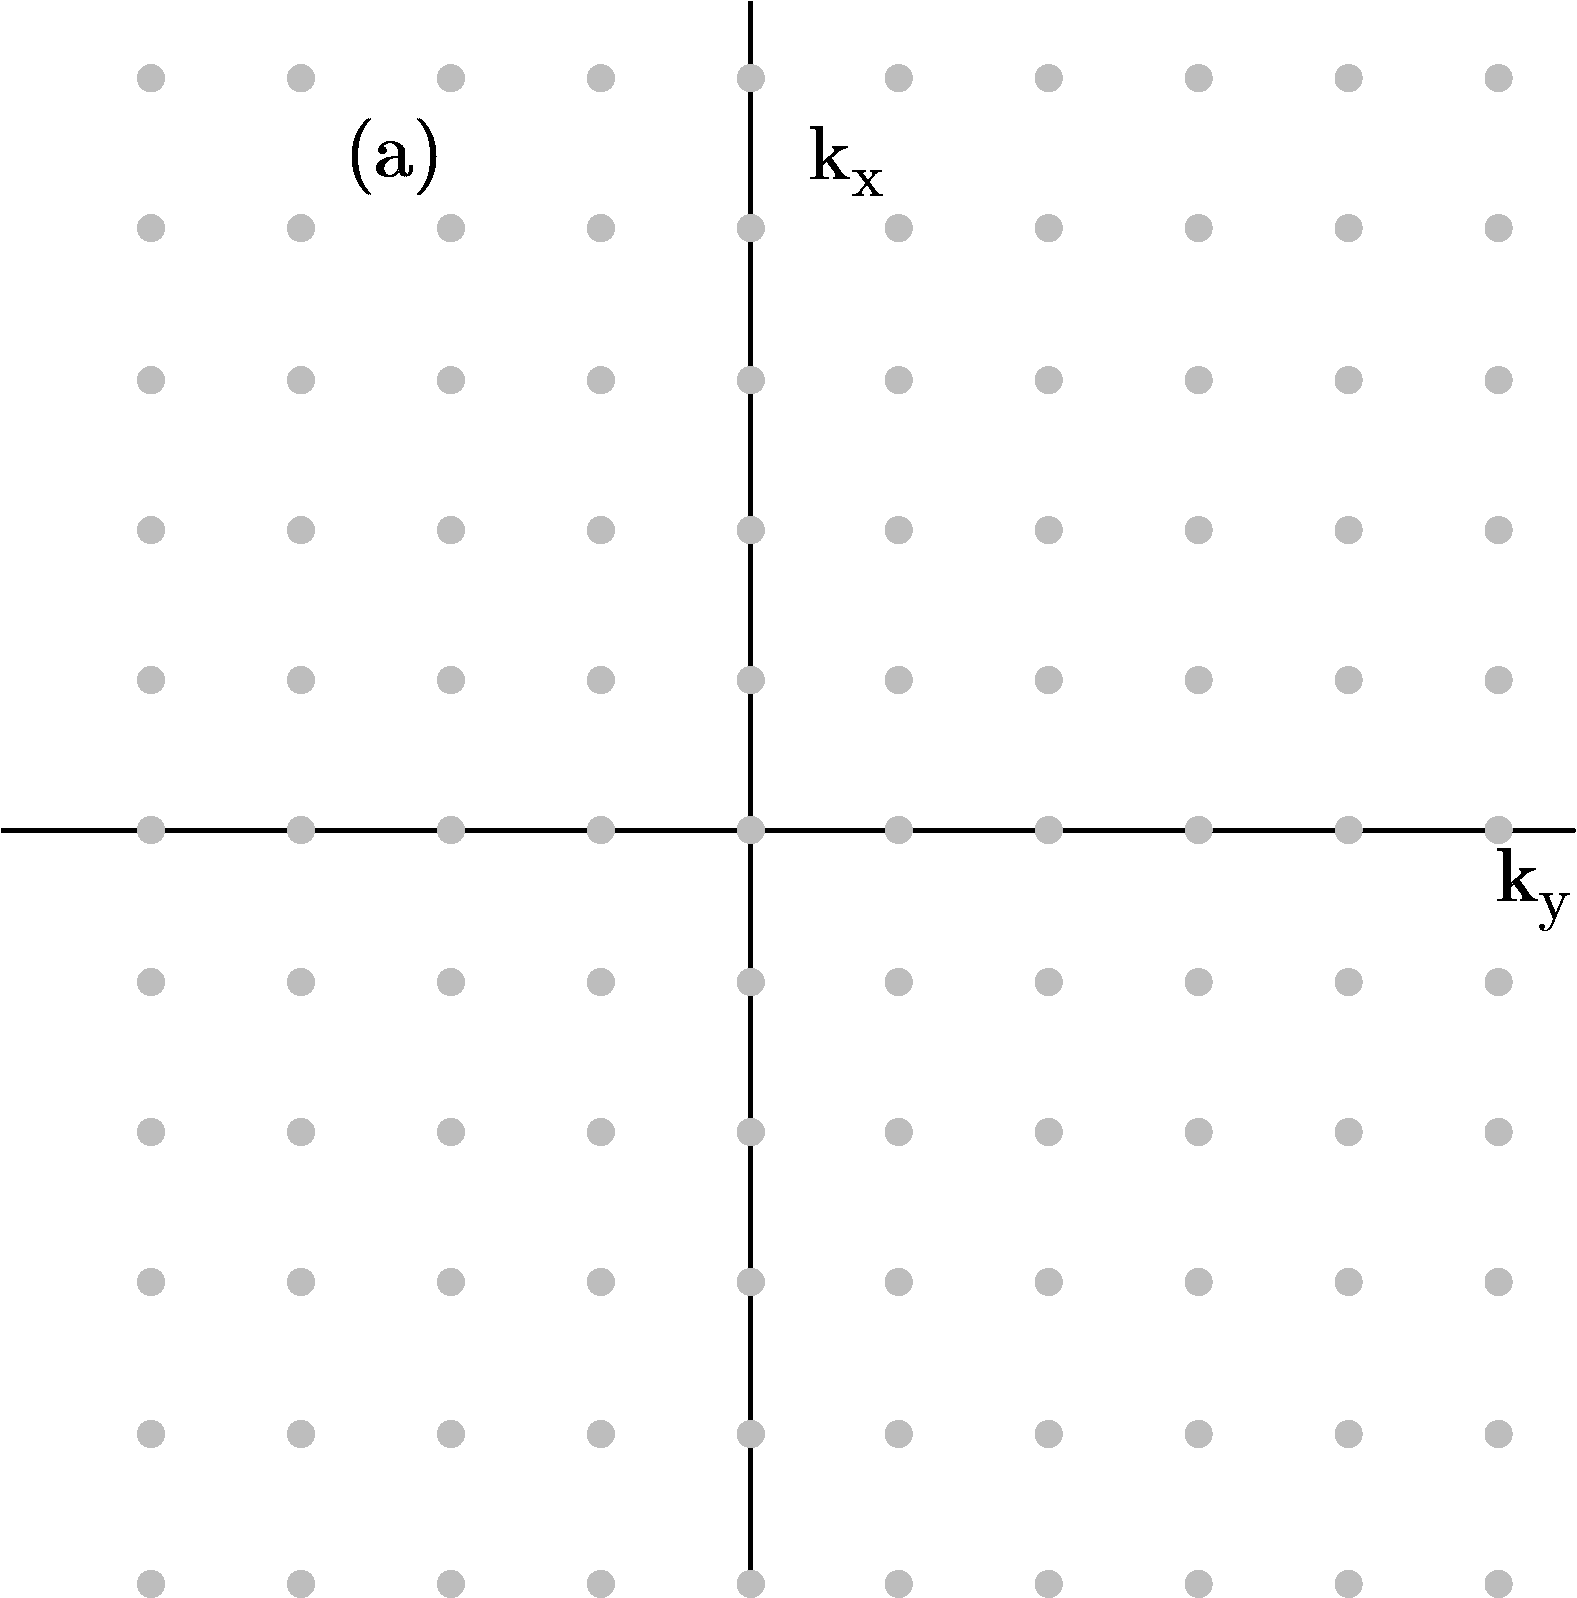
\includegraphics[width=0.8\linewidth]{script_figs/square_orbit.pdf}
	\end{subfigure}
	\begin{subfigure}{0.495\textwidth}
		\centering
		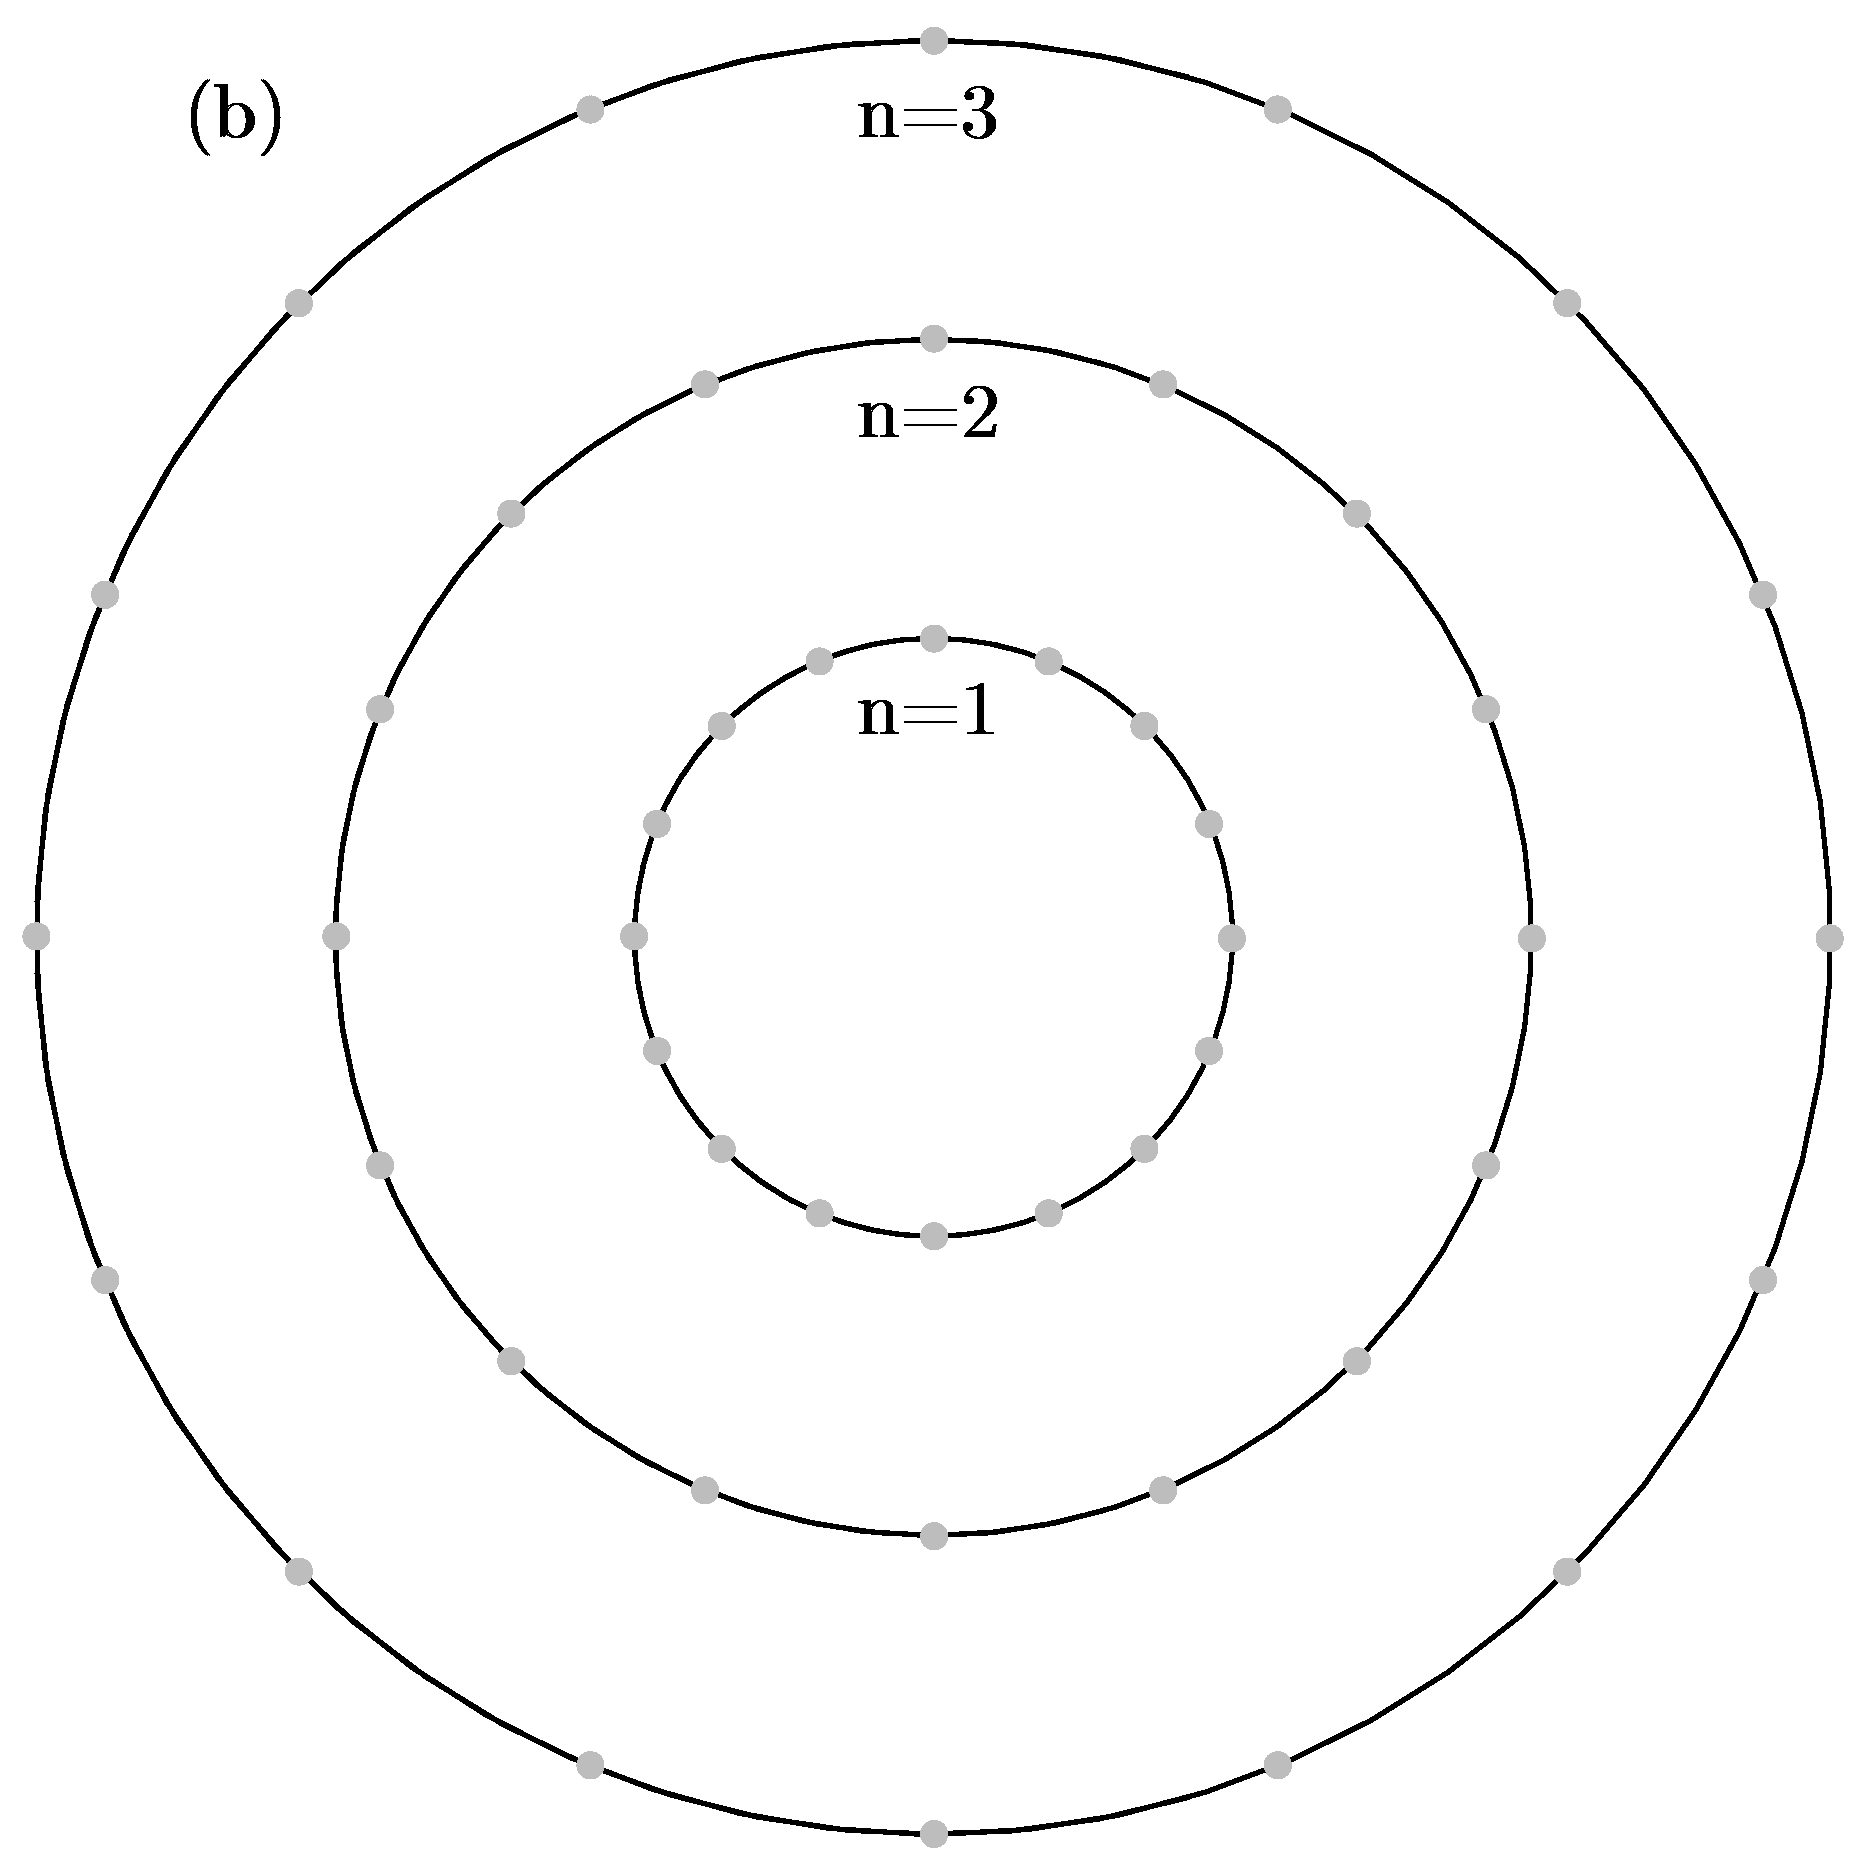
\includegraphics[width=0.8\linewidth]{script_figs/circle_orbit.pdf}
	\end{subfigure}
	\caption{(a) Electron motion in two dimensions without magnetic field. (b) Under magnetic field, electrons move in circular orbits in the ${k}$-plane.}
\end{figure}

When an electron moves in a periodic crystal lattice under a magnetic field $B$, its motion is governed by two distinct types of periodic dynamics. The first originates from the periodic lattice potential, while the second is the cyclotron motion induced by the Lorentz force, which drives the electron into circular orbits with a cyclotron radius $r_{c} \propto \frac{1}{B}$. At weak magnetic fields, the cyclotron radius $r_{c}$ is much larger than the lattice constant $a$. In this regime, the two motions---lattice periodic motion and cyclotron motion---are essentially independent, and the effective mass $m^{*}$ remains nearly constant. At strong magnetic fields, however, the cyclotron radius $r_{c}$ becomes comparable to the lattice constant $r_{0}$. Consequently, the electron dynamics are strongly influenced by the interplay between the Lorentz force and the periodic lattice potential. This coupling gives rise to a variety of rich physical phenomena, such as the Hofstadter butterfly, where the Landau levels form a fractal-like structure, and modifications of the effective mass $m^{*}$. These effects may exhibit distinct behaviors in the $K$ and $K'$ valleys.

\begin{table}[!h]
	\centering
	\renewcommand{\arraystretch}{2.0}
	\begin{tabular}{c c c | c c c}
		\hline\hline
		                      & $\hbar v_{F}$ (eV\AA) & $v_{F}$ (m/s)        &                      & $\hbar v_{F}$ (eV\AA) & $v_{F}$ (m/s)        \\
		\hline
		MoS\textsubscript{2}  & 2.76                  & 4.19 $\times 10^{5}$ & WS\textsubscript{2}  & 4.38                  & 6.65 $\times 10^{5}$ \\ \hline
		MoSe\textsubscript{2} & 2.53                  & 3.84 $\times 10^{5}$ & WSe\textsubscript{2} & 3.94                  & 5.99 $\times 10^{5}$ \\ \hline
		MoTe\textsubscript{2} & 0.87                  & 1.32 $\times 10^{5}$ & WTe\textsubscript{2} & 2.03                  & 3.09 $\times 10^{5}$ \\
		\hline\hline
	\end{tabular}
	\caption{Parameters of the effective Hamiltonian for the four common types of TMDs. The Fermi velocities are taken from Ref.~\cite{have2019,luo2016}.}
\end{table}

\newpage

\section{Methods}

When a magnetic field is applied to the crystal lattice, the magnetic unit cell is enlarged $q$ times for square lattice ($2q$ times for hexagonal lattice). As a consequence, the magnetic Brillouin zone smaller $2q$ times than the orginal Brillouin zone \cite{xiao2010}. 

In addition, the three bases $d_{z^{2}}, d_{xy}, d_{x^{2}-y^{2}}$, which were introduced by Liu \textit{et al.}, cannot clearly distinguish the $K$ and $K'$ points in the valence and conduction bands for two reasons. First, the squared amplitudes $|\psi|^{2}$ are identical. Second, in the magnetic Brillouin zone, the $K$ and $K'$ valleys cannot be intuitively distinguished by the dispersion relation $E(\mathbf{k})$; instead, one needs to examine the properties of the wave functions. Specifically, the electron wave function at the $K$ valley in conduction band is mainly contributed by $d_{z^{2}}$, while at the valence band it is $d_{xy} + d_{x^{2}-y^{2}}$. Furthemore, we can distingushed $K$ and $K'$ valleys at the valence by using bases
\begin{gather}
	\ket{\psi_{v}^{K}} = \frac{1}{\sqrt{2}} \left( \ket{d_{x^{2} - y^{2}}} + i \ket{d_{xy}} \right),\\
	\ket{\psi_{v}^{K'}} = \frac{1}{\sqrt{2}} \left( \ket{d_{x^{2} - y^{2}}} - i \ket{d_{xy}} \right).
\end{gather}
Therefore, it is necessary to adopt another basis set. We now consider a new basis consisting of the three eigenfunctions of the angular momentum operators $L^{2}$ and $L_{z}$, corresponding to $l = 2$ and $m = 0, \pm 2$.

\begin{gather}
	\ket{\tilde{\phi}_{1}} = \ket{d_{m = 0}}, \quad
	\ket{\tilde{\phi}_{2}} = \ket{d_{m = +2}}, \quad
	\ket{\tilde{\phi}_{3}} = \ket{d_{m = -2}}.
\end{gather}
The new basis can be obtained from the old one by the transformation
\begin{gather}
	\ket{\tilde{\phi}_{j}} = \sum_{j'} W_{j'j} \ket{\phi_{j'}},
\end{gather}
where
\begin{gather}
	W =
	\begin{pNiceMatrix}
		1 & 0                  & 0                   \\
		0 & \frac{i}{\sqrt{2}} & -\frac{i}{\sqrt{2}} \\
		0 & \frac{1}{\sqrt{2}} & \frac{1}{\sqrt{2}}
	\end{pNiceMatrix}.
\end{gather}
In particular,
\begin{gather}
	\ket{\tilde{\phi}_{1}} = \ket{\phi_{1}},\\
	\ket{\tilde{\phi}_{2}} = \frac{i}{\sqrt{2}} \ket{\phi_{2}} + \frac{1}{\sqrt{2}} \ket{\phi_{3}},\\
	\ket{\tilde{\phi}_{3}} = -\frac{i}{\sqrt{2}} \ket{\phi_{2}} + \frac{1}{\sqrt{2}} \ket{\phi_{3}}.
\end{gather}
The TB Hamiltonian in new basis reads
\begin{equation}
	\begin{aligned}
		\tilde{H}^{\text{TB}} (\mathbf{k}) & = W^{\dagger} H^{\text{TB}}(\mathbf{k}) W,
	\end{aligned}
\end{equation}
where $H^{\text{TB}} = H^{\text{NN}}$ or $H^{\text{TNN}}$.

To distinguish the states that originate from the original Brillouin zone, we follow the convention of Ho \textit{et al.}~\cite{ho2014}. Each Landau level is then labeled as $\ket{j, n}_{\tau}$, where $j$, $n$, and $\tau$ denote the orbital, Landau, and valley indices, respectively.

\textbf{Degeneracy:} The degeneracy of Landau levels can be addressed by two reasons, first arises from the motion of electrons in a 2D system and second comes from the magnetic Brillouin zone.
We have known that the magnetic Brillouin zone is $2q$ smaller than the orginal one. When magnetic field is turned on, we might obtained at least doublet degeneracy in Landau level. Second, in the absence of magnetic field, electron moving in periodic lattice crystal, but when a magnetic field is applied, electrons follow circular orbits (see in Fig.~2(a)). Here the Lorentz force are dominant, and the lattice potential is considered as slightly perturbation. Due to translational symmetry, these orbits can be positioned anywhere within the sample without changing their energy \cite{kittel2018}. 

\begin{figure}[htb]
	\begin{subfigure}{0.495\textwidth}
		\centering
		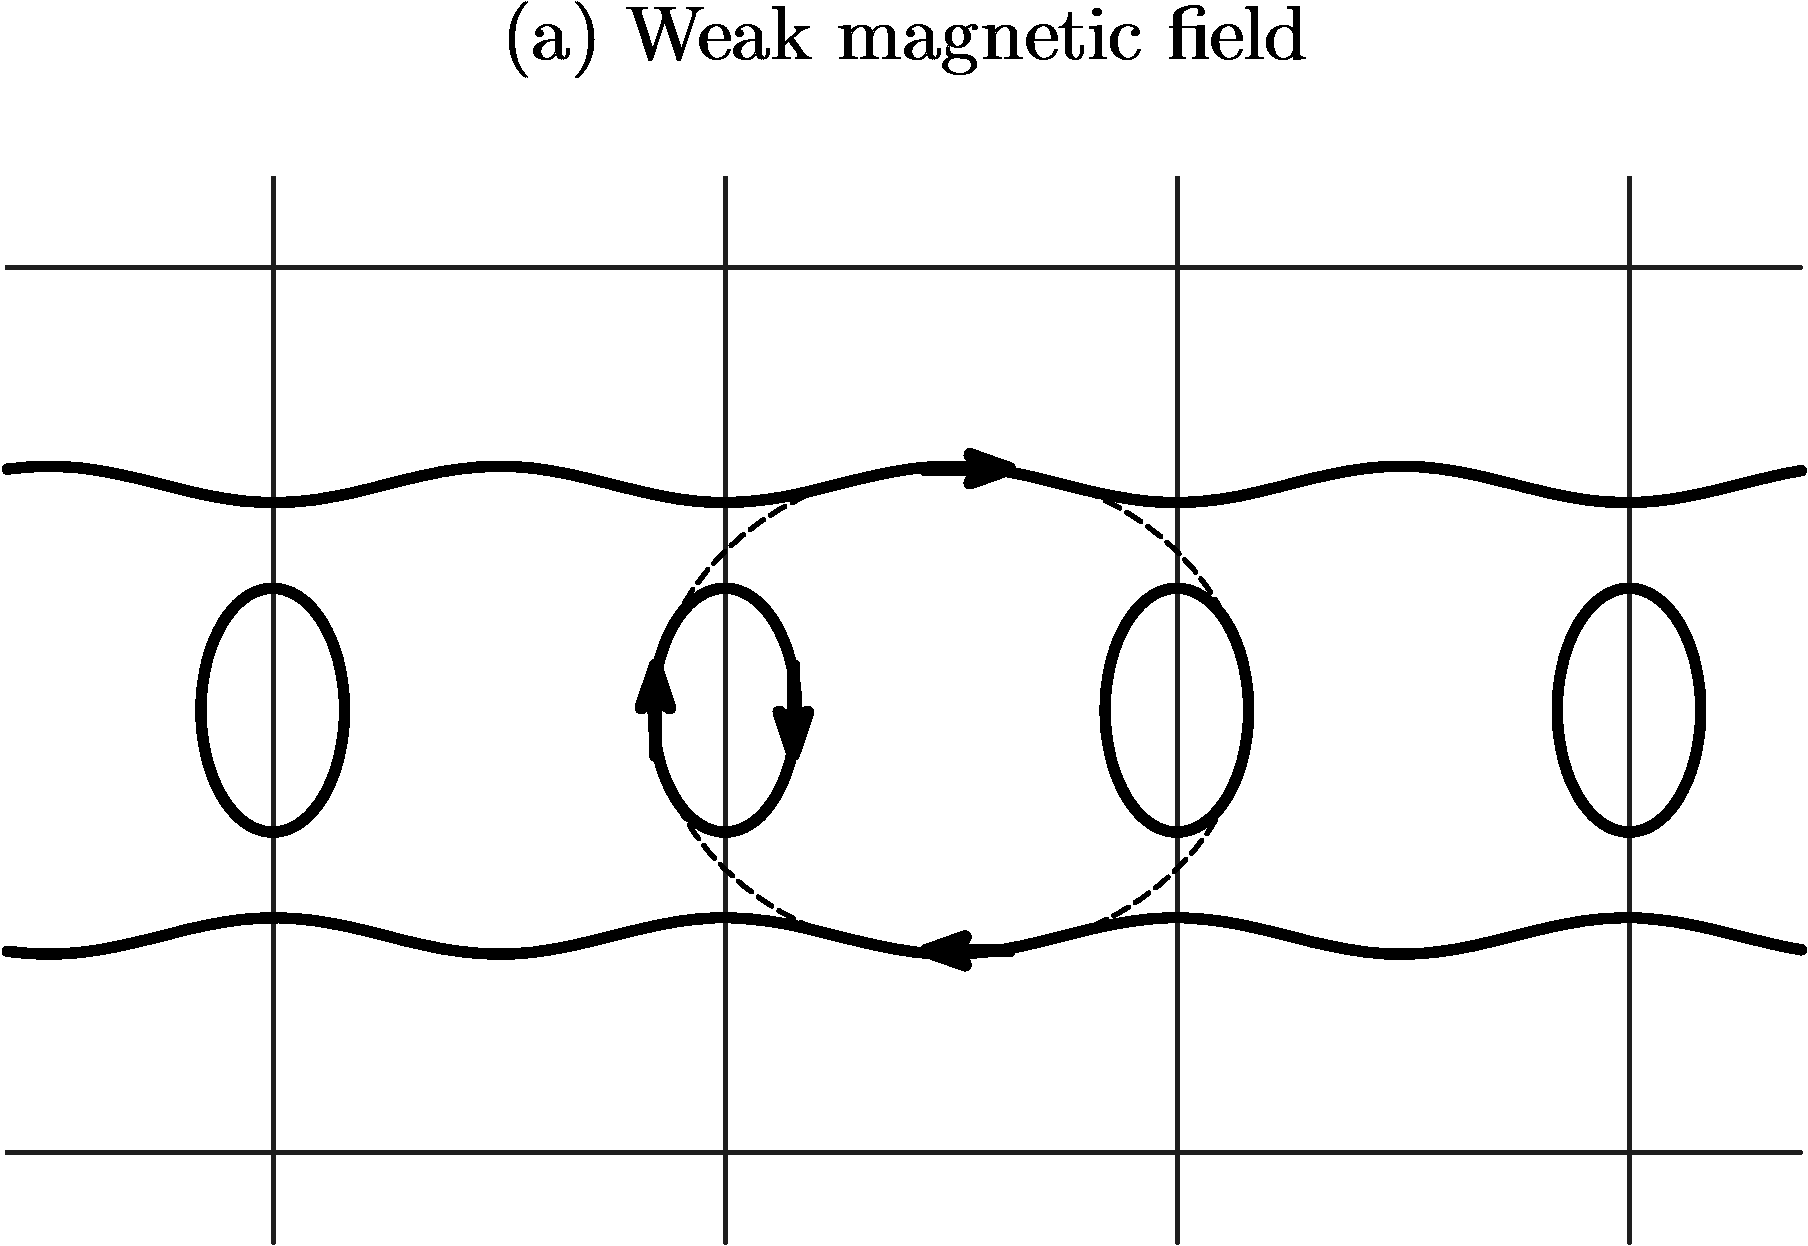
\includegraphics[width=\linewidth]{script_figs/weak_BZ.pdf}
	\end{subfigure}
	\begin{subfigure}{0.495\textwidth}
		\centering
		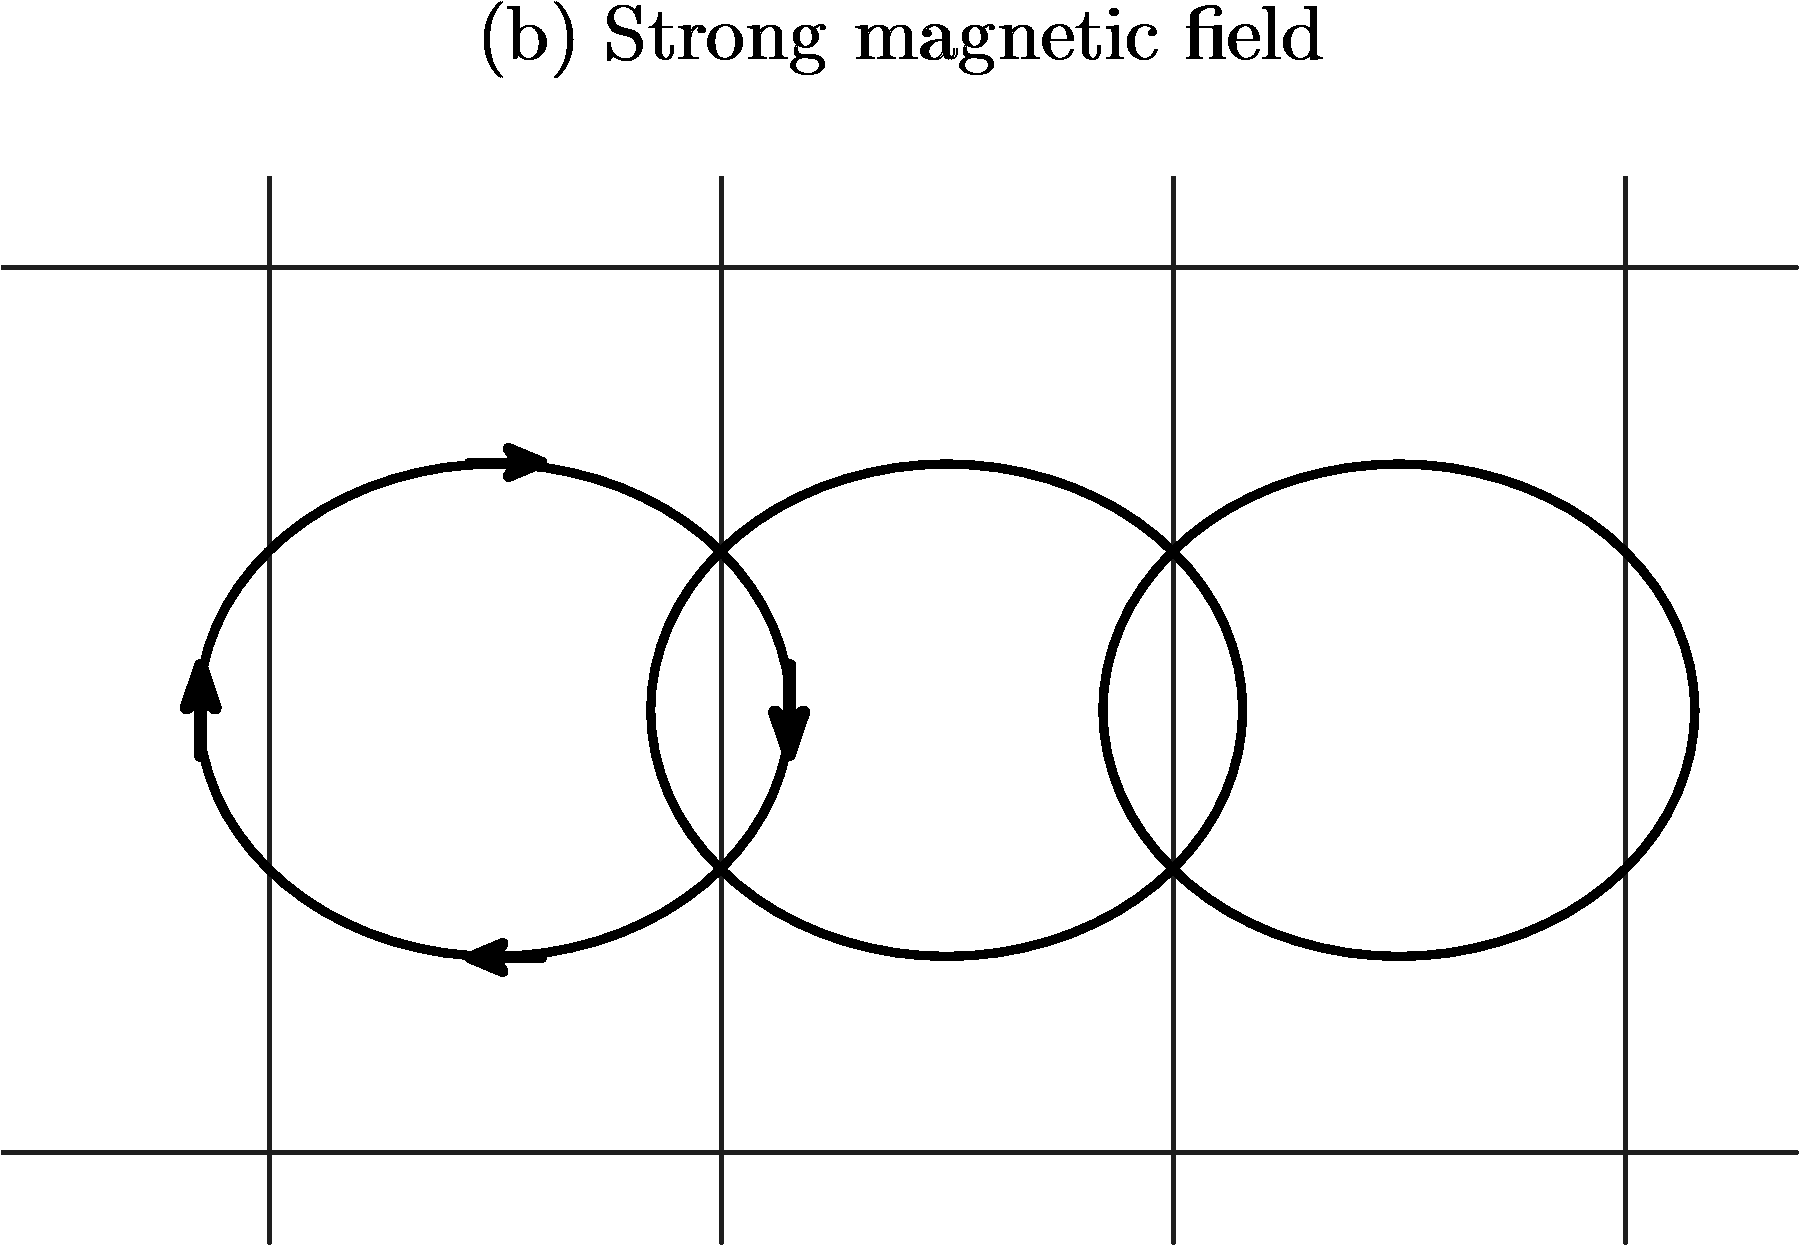
\includegraphics[width=\linewidth]{script_figs/strong_BZ.pdf}
	\end{subfigure}
	\caption{Periodic zone scheme, adapted from Kittel \textit{et al.}~\cite{kittel2018}. The straight lines indicate the Brillouin zones, the curved lines in (a) represent the band structure, and the elliptical lines correspond to the cyclotron orbits.}
\end{figure}

When diagonalizing the Hamiltonian in Eq.~(14), we obtain $2q$ eigenvalues for each orbital $\phi_{j}(\mathbf{r})$, with $j = 1,2,3$. In total, this gives $6q$ eigenvalues. The eigenvalues corresponding to the valence band range from $1$ to $2q$, while those of the conduction band range from $2q+1$ to $4q$.

For instance, in Fig.~3(a), the first Landau level is labeled as $\ket{0,0}_{K'}$. This level is degenerate, i.e., $E_{2q+1} = E_{2q+2}$, corresponding to the same energy value. Similarly, the second Landau level is labeled as $\ket{0,1}_{K'}$, which corresponds to the two degenerate eigenvalues $E_{2q+3} = E_{2q+4}$, and so on for the subsequent Landau levels. In Fig.~3(e), for the valence band, we clearly observe the evidence of the Brillouin zone shrinking. At a given value of $B$, the energy value is obtained simultaneously at the $K$, $K'$ and $\Gamma$ points. The first Landau level in the valence band corresponds to the eigenvalue $E_{2q}$ (labeled as $\ket{0,0}_{\Gamma}$), which is degenerate with $E_{2q-1}$. The second Landau level then corresponds to $E_{2q-2}$ and $E_{2q-3}$, and so on for the lower levels. 

In terms of Eq.~(18), we have
\begin{equation}
	\begin{aligned}
		m_{e}^{*} & = \frac{e B \hbar}{E_{2q+3} - E_{2q+1}}.
	\end{aligned}
\end{equation}
However, for $m_{h}^{*}$, the situation is quite different and more complicated than for $m_{e}^{*}$. For some cases, like MoS$_{2}$, this difficulty arises because the energy of the $\Gamma$ point lies close to the $K$ and $K'$ valleys.
As a consequence, in Fig.~1(d), the eigenvalues are no longer linear or follow the sequential index $2q-n$ as in the case of $m_{e}^{*}$, but instead exhibit level crossings due to numerical issues.
To address this, first, we need to determine the energy value $E_{n}$ at a given $B$ that corresponds to the envelope function.
This can be done by plotting all the wave functions from $0$ to $2q$, since each wave function provides information about the Landau level labeling.
From the wave functions, we can then identify which $E_{n}$ corresponds to $\ket{j,n}_{\tau}$.



\newpage
\section{Numerical results}
\subsection{Effective mass}
\subsubsection*{Monolayer MoS$_{2}$}

\begin{figure}[htb]
	\begin{subfigure}{0.495\textwidth}
		\centering
		\includegraphics[width=\linewidth]{imgs/MoS2/ButAndWave_c.pdf}
	\end{subfigure}
	\begin{subfigure}{0.495\textwidth}
		\centering
		\includegraphics[width=\linewidth]{imgs/MoS2/ButAndWave_v.pdf}
	\end{subfigure}
	\caption{Landau levels (a) and the corresponding envelope-function components (b),(c),(d) for conduction electrons at valleys $K$ and $K'$. Figs (e)–(h) show the same as (a)–(d) but for valence electrons. (Recalculated from Ho \textit{et al.} \cite{ho2014})}
\end{figure}
\begin{figure}[!h]
	\begin{subfigure}{0.495\textwidth}
		\centering
		\includegraphics[width=\linewidth]{imgs/MoS2/ButAndWave_cTNN.pdf}
	\end{subfigure}
	\begin{subfigure}{0.495\textwidth}
		\centering
		\includegraphics[width=\linewidth]{imgs/MoS2/ButAndWave_vTNN.pdf}
	\end{subfigure}
	\caption{Same as Figure~1 but for TNN case.}
\end{figure}

The band structure of MoS$_{2}$ without a magnetic field shows that, in the valence band, the $\Gamma$ point has an energy level of $E \approx -0.058$ eV. Therefore, when a magnetic field is applied, this $\Gamma$-point energy level still appears. The Landau levels in conduction band are mainly contributed by the basis $\ket{0}$. In the valence band, the $\Gamma$, $K$, and $K'$ points can be easily identified by their weights in the wavefunction. However, the situation is opposite in the conduction band. In this work, we adopt the results from the previous studies by Have \textit{et al.} and Korm{\'a}nyos \textit{et al.} \cite{have2019,kormanyos2015landau}. They shown that, in the conduction band the lowest Landau level is in valley $K$, while in valence band it is in valley $K'$.

The effective masses of MoS$_{2}$ in the absence of a magnetic field, calculated from
\begin{gather}
	\frac{1}{m_{ij}^{*}} = \frac{1}{\hbar^{2}} \frac{\partial^{2} E(\mathbf{k})}{\partial k_{i}\partial k_{j}},
\end{gather}
are $m_{e} \approx 0.4178 m_{0}$, $m_{h} \approx 0.5325 m_{0}$, and $m_{r} \approx 0.2341$ for the TNN case, and $m_{e} \approx 0.4508 m_{0}$, $m_{h} \approx 0.6487 m_{0}$, and $m_{r} \approx 0.2659 m_{0}$ for the NN case.

\begin{figure}[!h]
	\begin{subfigure}{0.495\textwidth}
		\centering
		\includegraphics[width=\linewidth]{imgs/MoS2/massK1.pdf}
	\end{subfigure}
	\begin{subfigure}{0.495\textwidth}
		\centering
		\includegraphics[width=\linewidth]{imgs/MoS2/massK2.pdf}
	\end{subfigure}
	\caption{Effective masses.}
\end{figure}
When a strong magnetic field is applied, for example $B = 100$ T:

\begin{itemize}
	\item[a)] Nearest neighbor (NN)
	      \begin{itemize}
		      \item At valley $K$: $m_{h} \approx 0.7011 m_{0},\; m_{e} \approx 0.4763 m_{0}$.
		            The reduced mass is $m_{r} \approx 0.2836 m_{0}$, which increases by $\approx 6.7\%$.

		      \item At valley $K'$: $m_{h} \approx 0.6597 m_{0},\; m_{e} \approx 0.4606 m_{0}$.
		            The reduced mass is $m_{r} \approx 0.2713 m_{0}$, which increases by $\approx 2.0\%$.
	      \end{itemize}
	\item[b)] Third nearest neighbor (TNN)
	      \begin{itemize}
		      \item At valley $K$: $m_{h} \approx 0.5739 m_{0},\; m_{e} \approx 0.4573 m_{0}$.
		            The reduced mass is $m_{r} \approx 0.2545 m_{0}$, which increases by $\approx 8.71\%$.

		      \item At valley $K'$: $m_{h} \approx 0.5584 m_{0},\; m_{e} \approx 0.4263 m_{0}$.
		            The reduced mass is $m_{r} \approx 0.2417 m_{0}$, which increases by $\approx 3.25\%$.
	      \end{itemize}
\end{itemize}


Meanwhile, Goryca \textit{et al.} \cite{goryca2019} reported that $m_{r} \approx 0.27 \pm 0.01 m_{0}$, which is $4\%-10.2\%$ larger than the earlier result of Berkelbach \textit{et al.} \cite{berkelbach2013}, $m_{r} = 0.245 \pm 0.005 m_{0}$.
Based on our calculations, we argue that the reduced mass at valley $K$, $m_{r} \approx 0.2545 m_{0}$ with an increase of $8.71\%$, is consistent with the experimental findings of Goryca \textit{et al.}

\begin{figure}[!h]
	\begin{subfigure}{0.495\textwidth}
		\centering
		\includegraphics[width=\linewidth]{imgs/MoS2/radiusK1.pdf}
	\end{subfigure}
	\begin{subfigure}{0.495\textwidth}
		\centering
		\includegraphics[width=\linewidth]{imgs/MoS2/radiusK2.pdf}
	\end{subfigure}
	\caption{The ratio of the cyclotron radius $r_c$ to the lattice constant $a$ as a function of magnetic field $B$.}
\end{figure}




\newpage
\subsubsection*{Monolayer MoSe$_{2}$}
\begin{figure}[htb]
	\begin{subfigure}{0.495\textwidth}
		\centering
		\includegraphics[width=\linewidth]{imgs/MoSe2/ButAndWave_c.pdf}
	\end{subfigure}
	\begin{subfigure}{0.495\textwidth}
		\centering
		\includegraphics[width=\linewidth]{imgs/MoSe2/ButAndWave_v.pdf}
	\end{subfigure}
	\caption{Landau levels (a) and the corresponding envelope-function components (b),(c) for conduction electrons at valleys $K$ and $K'$. Figs (d)–(f) show the same as (a)–(c) but for valence electrons.}
\end{figure}

\begin{figure}[!h]
	\begin{subfigure}{0.495\textwidth}
		\centering
		\includegraphics[width=\linewidth]{imgs/MoSe2/ButAndWave_cTNN.pdf}
	\end{subfigure}
	\begin{subfigure}{0.495\textwidth}
		\centering
		\includegraphics[width=\linewidth]{imgs/MoSe2/ButAndWave_vTNN.pdf}
	\end{subfigure}
	\caption{Same as Figure but for TNN case.}
\end{figure}

The band structure of MoSe$_{2}$ without a magnetic field shows that the $\Gamma$ point does not appear near the $K$ point. Therefore, when a magnetic field is applied, the $\Gamma$-point energy level is absent in this region. In addition, the first three Landau levels originate from the $K'$ valley, in contrast to WSe$_{2}$, where the first two Landau levels originate from the $K'$ valley.

The effective masses of MoSe$_{2}$ in the absence of a magnetic field, calculated from
\begin{gather}
	\frac{1}{m_{ij}^{*}} = \frac{1}{\hbar^{2}} \frac{\partial^{2} E(\mathbf{k})}{\partial k_{i}\partial k_{j}},
\end{gather}
are $m_{e} \approx 0.4770 m_{0}$, $m_{h} \approx 0.5887 m_{0}$, and $m_{r} \approx 0.2634 m_{0}$ for the TNN case, and $m_{e} \approx 0.5226 m_{0}$, $m_{h} \approx 0.7512 m_{0}$, and $m_{r} \approx 0.3082 m_{0}$ for the NN case.

When a strong magnetic field is applied, for example $B = 100$ T:

\begin{itemize}
	\item[a)] Nearest neighbor (NN)
	      \begin{itemize}
		      \item At valley $K$: $m_{h} \approx 0.8100 m_{0},\; m_{e} \approx 0.5529 m_{0}$.
		            The reduced mass is $m_{r} \approx 0.3286 m_{0}$, which increases by $\approx 6.62\%$.

		      \item At valley $K'$: $m_{h} \approx 0.7632 m_{0},\; m_{e} \approx 0.5331 m_{0}$.
		            The reduced mass is $m_{r} \approx 0.3138 m_{0}$, which increases by $\approx 1.82\%$.
	      \end{itemize}
	\item[b)] Third nearest neighbor (TNN)
	      \begin{itemize}
		      \item At valley $K$: $m_{h} \approx 0.7168 m_{0},\; m_{e} \approx 0.5320 m_{0}$.
		            The reduced mass is $m_{r} \approx 0.3052 m_{0}$, which increases by $\approx 15.87\%$.

		      \item At valley $K'$: $m_{h} \approx 0.6251 m_{0},\; m_{e} \approx 0.4874 m_{0}$.
		            The reduced mass is $m_{r} \approx 0.2738 m_{0}$, which increases by $\approx 3.95\%$.
	      \end{itemize}
\end{itemize}

\begin{figure}[htb]
	\begin{subfigure}{0.495\textwidth}
		\centering
		\includegraphics[width=\linewidth]{imgs/MoSe2/massK1.pdf}
	\end{subfigure}
	\begin{subfigure}{0.495\textwidth}
		\centering
		\includegraphics[width=\linewidth]{imgs/MoSe2/massK2.pdf}
	\end{subfigure}
	\caption{Effective masses.}
\end{figure}
\begin{figure}[!h]
	\begin{subfigure}{0.495\textwidth}
		\centering
		\includegraphics[width=\linewidth]{imgs/MoSe2/radiusK1.pdf}
	\end{subfigure}
	\begin{subfigure}{0.495\textwidth}
		\centering
		\includegraphics[width=\linewidth]{imgs/MoSe2/radiusK2.pdf}
	\end{subfigure}
	\caption{The ratio of the cyclotron radius $r_c$ to the lattice constant $a$ as a function of magnetic field $B$.}
\end{figure}

Meanwhile, Goryca \textit{et al.} \cite{goryca2019} reported that $m_{r} \approx 0.350 \pm 0.015 m_{0}$, which is $24.1\%-35.2\%$ larger than the earlier result of Berkelbach \textit{et al.} \cite{berkelbach2013}, $m_{r} = 0.27 m_{0}$.
Based on our calculations, we argue that at valley $K$, the reduced mass $m_{r} \approx 0.3052 m_{0}$, with an increase of $15.87\%$, does not fully agree with the experimental findings of Goryca \textit{et al.}.






\newpage
\subsubsection*{Monolayer MoTe$_{2}$}
\begin{figure}[htb]
	\begin{subfigure}{0.495\textwidth}
		\centering
		\includegraphics[width=\linewidth]{imgs/MoTe2/ButAndWave_c.pdf}
	\end{subfigure}
	\begin{subfigure}{0.495\textwidth}
		\centering
		\includegraphics[width=\linewidth]{imgs/MoTe2/ButAndWave_v.pdf}
	\end{subfigure}
	\caption{Landau levels (a) and the corresponding envelope-function components (b),(c) for conduction electrons at valleys $K$ and $K'$. Figs (d)–(f) show the same as (a)–(c) but for valence electrons.}
\end{figure}
\begin{figure}[!h]
	\begin{subfigure}{0.495\textwidth}
		\centering
		\includegraphics[width=\linewidth]{imgs/MoTe2/ButAndWave_cTNN.pdf}
	\end{subfigure}
	\begin{subfigure}{0.495\textwidth}
		\centering
		\includegraphics[width=\linewidth]{imgs/MoTe2/ButAndWave_vTNN.pdf}
	\end{subfigure}
	\caption{Landau levels (a) and the corresponding envelope-function components (b),(c) for conduction electrons at valleys $K$ and $K'$. Figs (d)–(f) show the same as (a)–(c) but for valence electrons.}
\end{figure}
The band structure of MoTe$_{2}$ without a magnetic field shows that the $\Gamma$ point has an energy level of $E \approx -0.1075$ eV. Therefore, when a magnetic field is applied, this $\Gamma$-point energy level not appears.

The effective masses of MoTe$_{2}$ in the absence of a magnetic field, calculated from
\begin{gather}
	\frac{1}{m_{ij}^{*}} = \frac{1}{\hbar^{2}} \frac{\partial^{2} E(\mathbf{k})}{\partial k_{i}\partial k_{j}},
\end{gather}
are $m_{e} \approx 0.4318 m_{0}$, $m_{h} \approx 0.6044 m_{0}$, and $m_{r} \approx 0.2519 m_{0}$ for the TNN case, and $m_{e} \approx 0.5913 m_{0}$, $m_{h} \approx 0.8975 m_{0}$, and $m_{r} \approx 0.3565 m_{0}$ for the NN case, as also reported by Goryca \textit{et al.} \cite{goryca2019}. Among the six materials considered, MoTe$_{2}$ has the largest effective masses $m_{e}$ and $m_{h}$ in the absence of a magnetic field.

When a strong magnetic field is applied, for example $B = 90$ T:

\begin{itemize}
	\item[a)] Nearest neighbor (NN)
	      \begin{itemize}
		      \item At valley $K$: $m_{h} \approx 0.9774 m_{0},\; m_{e} \approx 0.6304 m_{0}$.
		            The reduced mass is $m_{r} \approx 0.3832 m_{0}$, which increases by $\approx 7.49\%$.

		      \item At valley $K'$: $m_{h} \approx 0.9142 m_{0},\; m_{e} \approx 0.6034 m_{0}$.
		            The reduced mass is $m_{r} \approx 0.3635 m_{0}$, which increases by $\approx 1.96\%$.
	      \end{itemize}
	\item[b)] Third nearest neighbor (TNN)
	      \begin{itemize}
		      \item At valley $K$: $m_{h} \approx 0.7704 m_{0},\; m_{e} \approx 0.4850 m_{0}$.
		            The reduced mass is $m_{r} \approx 0.2976 m_{0}$, which increases by $\approx 18.14\%$.

		      \item At valley $K'$: $m_{h} \approx 0.6322 m_{0},\; m_{e} \approx 0.4463 m_{0}$.
		            The reduced mass is $m_{r} \approx 0.2616 m_{0}$, which increases by $\approx 3.85\%$.
	      \end{itemize}
\end{itemize}

\begin{figure}[htb]
	\begin{subfigure}{0.495\textwidth}
		\centering
		\includegraphics[width=\linewidth]{imgs/MoTe2/massK1.pdf}
	\end{subfigure}
	\begin{subfigure}{0.495\textwidth}
		\centering
		\includegraphics[width=\linewidth]{imgs/MoTe2/massK2.pdf}
	\end{subfigure}
	\caption{Effective masses.}
\end{figure}
\begin{figure}[!h]
	\begin{subfigure}{0.495\textwidth}
		\centering
		\includegraphics[width=\linewidth]{imgs/MoTe2/radiusK1.pdf}
	\end{subfigure}
	\begin{subfigure}{0.495\textwidth}
		\centering
		\includegraphics[width=\linewidth]{imgs/MoTe2/radiusK2.pdf}
	\end{subfigure}
	\caption{Effective masses.}
\end{figure}

In the study of Goryca \textit{et al.} \cite{goryca2019}, the reduced mass was reported as $m_{r} = 0.36 \pm 0.04 m_{0}$, which is about 25\% larger than the value obtained in the work of Korm\'{a}nyos \textit{et al.} \cite{kormanyos2015}. In our case, for the TNN model, the reduced mass is $m_{r} = 0.2976 m_{0}$, which increases by $\approx 18\%$ compared to the zero-field value $m_{r} = 0.2519 m_{0}$.



\newpage
\subsubsection*{Monolayer WS$_{2}$}
\begin{figure}[htb]
	\begin{subfigure}{0.495\textwidth}
		\centering
		\includegraphics[width=\linewidth]{imgs/WS2/ButAndWave_c.pdf}
	\end{subfigure}
	\begin{subfigure}{0.495\textwidth}
		\centering
		\includegraphics[width=\linewidth]{imgs/WS2/ButAndWave_v.pdf}
	\end{subfigure}
	\caption{Landau levels (a) and the corresponding envelope-function components (b),(c) for conduction electrons at valleys $K$ and $K'$. Figs (d)–(f) show the same as (a)–(c) but for valence electrons.}
\end{figure}
\begin{figure}[!h]
	\begin{subfigure}{0.495\textwidth}
		\centering
		\includegraphics[width=\linewidth]{imgs/WS2/ButAndWave_cTNN.pdf}
	\end{subfigure}
	\begin{subfigure}{0.495\textwidth}
		\centering
		\includegraphics[width=\linewidth]{imgs/WS2/ButAndWave_vTNN.pdf}
	\end{subfigure}
	\caption{Landau levels (a) and the corresponding envelope-function components (b),(c) for conduction electrons at valleys $K$ and $K'$. Figs (d)–(f) show the same as (a)–(c) but for valence electrons.}
\end{figure}

The band structure of WS$_{2}$ without a magnetic field shows that the $\Gamma$ point has an energy level of $E \approx -0.1075$ (eV). Therefore, when a magnetic field is applied, the energy level at the $\Gamma$ point still appears.

The effective mass of WS$_{2}$ without a magnetic field, calculated using
\begin{gather}
	\frac{1}{m_{ij}^{*}} = \frac{1}{\hbar^{2}} \frac{\partial^{2} E(\mathbf{k})}{\partial k_{i} k_{j}},
\end{gather}
yields $m_{e} \approx 0.2956 m_{0},\; m_{h} \approx 0.3845 m_{0},\; m_{r} \approx 0.1671 m_{0}$ in the TNN case, and $m_{e} \approx 0.3195 m_{0},\; m_{h} \approx 0.4348 m_{0},\; m_{r} \approx 0.1841 m_{0}$ in the NN case.

For a strong magnetic field, e.g., $B = 100$ T:
\begin{itemize}
	\item[a)] Nearest neighbor
	      \begin{itemize}
		      \item At the K valley: $m_{h} \approx 0.4735 m_{0},\; m_{e} \approx 0.3389 m_{0}$. Thus, $m_{r} \approx 0.1974 m_{0}$, which increases by $\approx 7.2\%$.
		      \item At the K' valley: $m_{h} \approx 0.4438 m_{0},\; m_{e} \approx 0.3273 m_{0}$. Thus, $m_{r} \approx 0.1885 m_{0}$, which increases by $\approx 2.3\%$.
	      \end{itemize}
	\item[b)] Third nearest neighbor
	      \begin{itemize}
		      \item At the K valley: $m_{h} \approx 0.4205 m_{0},\; m_{e} \approx 0.3275 m_{0}$. Thus, $m_{r} \approx 0.1841 m_{0}$, which increases by $\approx 10.17\%$.
		      \item At the K' valley: $m_{h} \approx 0.4043 m_{0},\; m_{e} \approx 0.3023 m_{0}$. Thus, $m_{r} \approx 0.1730 m_{0}$, which increases by $\approx 3.53\%$.
	      \end{itemize}
\end{itemize}

In the study of Goryca \textit{et al.} \cite{goryca2019}, they reported $m_{r} = 0.175 \pm 0.007 m_{0}$, which is about 10\% larger than the value $m_{r} = 0.15 - 0.16 m_{0}$ obtained in the work of Berkelbach \textit{et al.} \cite{berkelbach2013}.

In our case, for the K valley under the TNN approximation, we obtain $m_{r} \approx 0.1841 m_{0}$ in the presence of a magnetic field, which corresponds to an increase of $\approx 10\%$ compared to $m_{r} \approx 0.1671 m_{0}$ without a magnetic field. This result is consistent with and reasonable compared to the experimental findings of Goryca \textit{et al.} \cite{goryca2019}.


\begin{figure}[htb]
	\begin{subfigure}{0.495\textwidth}
		\centering
		\includegraphics[width=\linewidth]{imgs/WS2/massK1.pdf}
	\end{subfigure}
	\begin{subfigure}{0.495\textwidth}
		\centering
		\includegraphics[width=\linewidth]{imgs/WS2/massK2.pdf}
	\end{subfigure}
	\caption{Mass.}
\end{figure}

\begin{figure}[!h]
	\begin{subfigure}{0.495\textwidth}
		\centering
		\includegraphics[width=\linewidth]{imgs/WS2/radiusK1.pdf}
	\end{subfigure}
	\begin{subfigure}{0.495\textwidth}
		\centering
		\includegraphics[width=\linewidth]{imgs/WS2/radiusK2.pdf}
	\end{subfigure}
	\caption{The ratio of the cyclotron radius $r_c$ to the lattice constant $a$ as a function of magnetic field $B$.}
\end{figure}
\newpage
\subsubsection*{Monolayer WSe$_{2}$}
\begin{figure}[htb]
	\begin{subfigure}{0.495\textwidth}
		\centering
		\includegraphics[width=\linewidth]{imgs/WSe2/ButAndWave_c.pdf}
	\end{subfigure}
	\begin{subfigure}{0.495\textwidth}
		\centering
		\includegraphics[width=\linewidth]{imgs/WSe2/ButAndWave_v.pdf}
	\end{subfigure}
	\caption{Landau levels (a) and the corresponding envelope-function components (b),(c) for conduction electrons at valleys $K$ and $K'$. Figs (d)–(f) show the same as (a)–(c) but for valence electrons.}
\end{figure}
\begin{figure}[!h]
	\begin{subfigure}{0.495\textwidth}
		\centering
		\includegraphics[width=\linewidth]{imgs/WSe2/ButAndWave_cTNN.pdf}
	\end{subfigure}
	\begin{subfigure}{0.495\textwidth}
		\centering
		\includegraphics[width=\linewidth]{imgs/WSe2/ButAndWave_vTNN.pdf}
	\end{subfigure}
	\caption{Landau levels (a) and the corresponding envelope-function components (b),(c) for conduction electrons at valleys $K$ and $K'$. Figs (d)–(f) show the same as (a)–(c) but for valence electrons.}
\end{figure}
The band structure of WSe$_{2}$ without a magnetic field shows that the $\Gamma$ point lies much lower in energy than the K point. Therefore, when a magnetic field is applied, the energy level at the $\Gamma$ point does not appear here.

The effective mass of WSe$_{2}$ without a magnetic field, calculated using
\begin{gather}
	\frac{1}{m_{ij}^{*}} = \frac{1}{\hbar^{2}} \frac{\partial^{2} E(\mathbf{k})}{\partial k_{i} k_{j}},
\end{gather}
yields $m_{e} \approx 0.3124 m_{0},\; m_{h} \approx 0.4022 m_{0},\; m_{r} \approx 0.1758 m_{0}$ in the TNN case, and $m_{e} \approx 0.3487 m_{0},\; m_{h} \approx 0.4792 m_{0},\; m_{r} \approx 0.2018 m_{0}$ in the NN case, as reported in the works of Kyl\"{a}np\"{a}\"{a} \textit{et al.} and Berkelbach \textit{et al.} \cite{berkelbach2013,kylanpaa2015}.

For a strong magnetic field, e.g., $B = 100$ T:
\begin{itemize}
	\item[a)] Nearest neighbor
	      \begin{itemize}
		      \item At the K valley: $m_{h} \approx 0.5220 m_{0},\; m_{e} \approx 0.3702 m_{0}$. Thus, $m_{r} \approx 0.2166 m_{0}$, which increases by $\approx 7.34\%$.
		      \item At the K' valley: $m_{h} \approx 0.4888 m_{0},\; m_{e} \approx 0.3573 m_{0}$. Thus, $m_{r} \approx 0.2064 m_{0}$, which increases by $\approx 2.28\%$.
	      \end{itemize}
	\item[b)] Third nearest neighbor
	      \begin{itemize}
		      \item At the K valley: $m_{h} \approx 0.4417 m_{0},\; m_{e} \approx 0.3494 m_{0}$. Thus, $m_{r} \approx 0.1951 m_{0}$, which increases by $\approx 10.98\%$.
		      \item At the K' valley: $m_{h} \approx 0.4257 m_{0},\; m_{e} \approx 0.3199 m_{0}$. Thus, $m_{r} \approx 0.1826 m_{0}$, which increases by $\approx 3.87\%$.
	      \end{itemize}
\end{itemize}

In the study of Stier \textit{et al.} \cite{stier2018}, they reported $m_{r} \approx 0.20 \pm 0.01 m_{0}$, which is about 15\% larger than the predictions of recent theoretical works \cite{berkelbach2013,kylanpaa2015}. In our case, for the K valley under the TNN approximation, we obtain $m_{r} \approx 0.1951 m_{0}$ in the presence of a magnetic field, corresponding to an increase of $\approx 11\%$ compared to the value without a magnetic field. This result is consistent with the findings reported by Stier \textit{et al.} \cite{stier2018}.

\begin{figure}[htb]
	\begin{subfigure}{0.495\textwidth}
		\centering
		\includegraphics[width=\linewidth]{imgs/WSe2/massK1.pdf}
	\end{subfigure}
	\begin{subfigure}{0.495\textwidth}
		\centering
		\includegraphics[width=\linewidth]{imgs/WSe2/massK2.pdf}
	\end{subfigure}
	\caption{Mass.}
\end{figure}
\begin{figure}[!h]
	\begin{subfigure}{0.495\textwidth}
		\centering
		\includegraphics[width=\linewidth]{imgs/WSe2/radiusK1.pdf}
	\end{subfigure}
	\begin{subfigure}{0.495\textwidth}
		\centering
		\includegraphics[width=\linewidth]{imgs/WSe2/radiusK2.pdf}
	\end{subfigure}
	\caption{The ratio of the cyclotron radius $r_c$ to the lattice constant $a$ as a function of magnetic field $B$.}
\end{figure}


\newpage
\subsubsection*{Monolayer WTe$_{2}$}
\begin{figure}[htb]
	\begin{subfigure}{0.495\textwidth}
		\centering
		\includegraphics[width=\linewidth]{imgs/WTe2/ButAndWave_c.pdf}
	\end{subfigure}
	\begin{subfigure}{0.495\textwidth}
		\centering
		\includegraphics[width=\linewidth]{imgs/WTe2/ButAndWave_v.pdf}
	\end{subfigure}
	\caption{Landau levels (a) and the corresponding envelope-function components (b),(c) for conduction electrons at valleys $K$ and $K'$. Figs (d)–(f) show the same as (a)–(c) but for valence electrons.}
\end{figure}
\begin{figure}[!h]
	\begin{subfigure}{0.495\textwidth}
		\centering
		\includegraphics[width=\linewidth]{imgs/WTe2/ButAndWave_c.pdf}
	\end{subfigure}
	\begin{subfigure}{0.495\textwidth}
		\centering
		\includegraphics[width=\linewidth]{imgs/WTe2/ButAndWave_vTNN.pdf}
	\end{subfigure}
	\caption{Landau levels (a) and the corresponding envelope-function components (b),(c) for conduction electrons at valleys $K$ and $K'$. Figs (d)–(f) show the same as (a)–(c) but for valence electrons.}
\end{figure}

The band structure of WTe$_{2}$ in the absence of a magnetic field shows that the $\Gamma$ point lies significantly lower in energy than the K point. Therefore, under an applied magnetic field, the Landau levels associated with the $\Gamma$ point do not appear in this regime.

The effective masses of WTe$_{2}$ without a magnetic field, calculated using the formula
\begin{gather}
	\frac{1}{m_{ij}^*} = \frac{1}{\hbar^{2}} \frac{\partial^{2}E(\mathbf{k})}{\partial k_{i} k_{j}},
\end{gather}
are found to be $m_{e} \approx 0.2478 m_{0}$, $m_{h} \approx 0.3332 m_{0}$, and $m_{r} \approx 0.1421 m_{0}$ for the TNN case, and $m_{e} \approx 0.3169 m_{0}$, $m_{h} \approx 0.4559 m_{0}$, and $m_{r} \approx 0.187 m_{0}$ for the NN case. To the best of our knowledge, no previous studies have reported the effective masses of WTe$_{2}$.

At a high magnetic field, for example $B = 80$ T, the effective masses are obtained as follows:

\begin{itemize}
	\item[a)] Nearest neighbor
	      \begin{itemize}
		      \item At the K valley: $m_{h} \approx 0.5093 m_{0},\; m_{e} \approx 0.3413 m_{0}$. \\
		            This yields $m_{r} \approx 0.2044 m_{0}$, corresponding to an increase of $\approx 9.3\%$.

		      \item At the K$'$ valley: $m_{h} \approx 0.4681 m_{0},\; m_{e} \approx 0.3264 m_{0}$. \\
		            This gives $m_{r} \approx 0.1923 m_{0}$, corresponding to an increase of $\approx 2.83\%$.
	      \end{itemize}
	\item[b)] Third nearest neighbor
	      \begin{itemize}
		      \item At the K valley: $m_{h} \approx 0.387 m_{0},\; m_{e} \approx 0.2824 m_{0}$. \\
		            This yields $m_{r} \approx 0.1633 m_{0}$, corresponding to an increase of $\approx 14.92\%$.

		      \item At the K$'$ valley: $m_{h} \approx 0.3562 m_{0},\; m_{e} \approx 0.2577 m_{0}$. \\
		            This gives $m_{r} \approx 0.1495 m_{0}$, corresponding to an increase of $\approx 5.21\%$.
	      \end{itemize}
\end{itemize}

Thus, at the K valley in the TNN case, the reduced mass $m_r$ of WTe$_{2}$ exhibits an increasing of nearly $15\%$ under a strong magnetic field, which is consistent with the trend observed for other materials discussed above.

\begin{figure}[htb]
	\begin{subfigure}{0.495\textwidth}
		\centering
		\includegraphics[width=\linewidth]{imgs/WTe2/massK1.pdf}
	\end{subfigure}
	\begin{subfigure}{0.495\textwidth}
		\centering
		\includegraphics[width=\linewidth]{imgs/WTe2/massK2.pdf}
	\end{subfigure}
	\caption{Mass.}
\end{figure}
\begin{figure}[!h]
	\begin{subfigure}{0.495\textwidth}
		\centering
		\includegraphics[width=\linewidth]{imgs/WTe2/radiusK1.pdf}
	\end{subfigure}
	\begin{subfigure}{0.495\textwidth}
		\centering
		\includegraphics[width=\linewidth]{imgs/WTe2/radiusK2.pdf}
	\end{subfigure}
	\caption{The ratio of the cyclotron radius $r_{c}$ to the lattice constant $a$ as a function of magnetic field $B$.}
\end{figure}

\newpage

\bibliographystyle{unsrt}
\bibliography{refs}

\end{document}
